%---------------------------------------------------------------------------%
\lecture{Research Presentation}{lec_present_sim}
%---------------------------------------------------------------------------%
\section{Simulation study}%
%---------------------------------------------------------------------------%
\begin{frame}[fragile]
    \frametitle{Measuring Prediction Performance}
    \begin{itemize}
        \item Selects the model that best fits the data.
        \item Bias-Variance Decomposition
        \begin{itemize}
            \item We carefully follow \cite{hastie2008elements}.
            \item Assume $Y=f(X) + \varepsilon$, where $E[\varepsilon]=0$ and $Var(\varepsilon)=\sigma^2_{\varepsilon}$
            \item We can derive the Mean Squared Error (MSE) out of the expected prediction error of $\hat{f}(X)$ at a \textbf{fixed} point $X = x_0$ 
            \begin{align}
            \label{}
            Err(x_0) &= E[(Y-\hat{f}(x_0))^2|X=x_0] \\
            &= \sigma^2_{\varepsilon} + [E\hat{f}(x_0) - f(x_0)]^2 + E[\hat{f}(x_0) - E\hat{f}(x_0)]^2 \\
            &= \sigma^2_{\varepsilon} + \: Bias^2(\hat{f}(x_0)) + Var(\hat{f}(x_0)) \\
            &= Irreducible \: error + \underbrace{\: Bias^2 + Variance}_\text{MSE}
            \end{align}
        \end{itemize}
    \end{itemize}
\end{frame}
%---------------------------------------------------------------------------%
\begin{frame}[fragile]
\frametitle{MSE as a Measurement of Model Fit}
    \begin{figure}[b]
        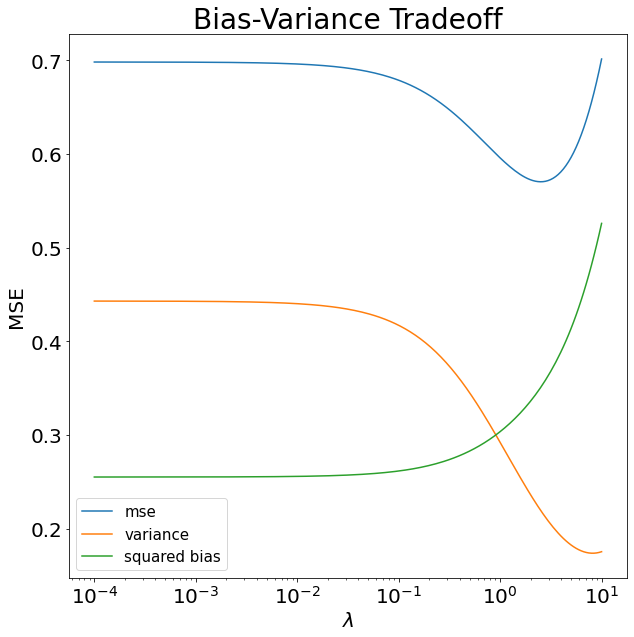
\includegraphics[scale=0.30]{Img/bias_var_tradeoff.png}%\hspace{-1.2cm}
        \centering
    \end{figure}
\end{frame}
%---------------------------------------------------------------------------%
\begin{frame}[fragile]
    \frametitle{DGP setup}
        $$
        y= X\beta + \varepsilon, \quad \text{with} \quad \varepsilon \sim \mathcal{N}_{n}(0, 1)
        $$

        $\textstyle X_{nxp} \sim \mathcal{N}(0, 1)$ such that the pairwise correlation between $x_{i}$ and $x_{j}$ is expressed as \\ 
        
        $$
        corr(\textit{i,j}) = \text{correlation factor} ^ \left|{i - j}\right|,
        $$\\ 
        
        where the correlation factor takes on a value between 0 and 1.
\end{frame}
%---------------------------------------------------------------------------%
\begin{frame}[fragile]
\frametitle{Minimum Test MSE (Case 1)}

\begin{block}{Set up}
    \begin{itemize}
        \item High dimensionality with varying sparsity, no multicollinearity. 
        \item $n = 30$
        \item $p = 35$
        \item All non-zero $\beta = 2$. 
    \end{itemize}
\end{block} \\

\begin{center}
    
    \begin{tabular}{||c c c c||} 
         \hline
          & High Sparsity & Med Sparsity & Low Sparsity \\ [0.5ex] 
          Model & (10 non-zero $\beta$'s) & (20 non-zero $\beta$'s) & (35 non-zero $\beta$'s) \\ [0.5ex]
         \hline\hline
         Ridge & 12.544 & 23.895 & \cellcolor{pink!60}36.074\\ 
         \hline
         Elnet (Naive), 0.2 & 10.182 & \cellcolor{pink!60}21.360 & 40.366 \\
         \hline
         Elnet (Naive), 0.5 & 8.760 & 21.687 & 46.961\\
        \hline
         Elnet (Naive), 0.7 & 7.421 & 22.380 & 52.046\\
        \hline
         Lasso & \cellcolor{pink!60}5.903 & 24.090 & 60.170\\
        \hline
    \end{tabular}

\end{center}
\end{frame}
%---------------------------------------------------------------------------%
\begin{frame}[fragile]
\frametitle{Minimum Test MSE (Case 2)}

\begin{block}{Set up}
    \begin{itemize}
        \item Low dimensionality with varying sparsity, moderate to high pairwise correlation (corr. factor = 0.8).  
        \item $n = 30$, $p = 10$
        \item All non-zero $\beta = 2$. 
    \end{itemize}
\end{block} \\

\begin{center}
    
    \begin{tabular}{||c c c c||} 
         \hline
          & High Sparsity & Med Sparsity & Low Sparsity \\ [0.5ex] 
          Model & (3 non-zero $\beta$'s) & (7 non-zero $\beta$'s) & (10 non-zero $\beta$'s) \\ [0.5ex]
         \hline\hline
         Ridge & 0.570 & 0.270 & \cellcolor{pink!60}1.140 \\ 
         \hline
         Elnet (Naive), 0.2 & 0.572 & 0.265 & 1.149 \\
         \hline
         Elnet (Naive), 0.5 & 0.577 & 0.246 & 1.164\\
        \hline
         Elnet (Naive), 0.7 & \cellcolor{pink!60}0.552 & \cellcolor{pink!60}0.218 & 1.166\\
        \hline
         Lasso & 0.607 & 0.298 & 1.166\\
        \hline
    \end{tabular}

\end{center}
\end{frame}
%---------------------------------------------------------------------------%
\begin{frame}[fragile]
\frametitle{Minimum Test MSE (Case 3)}

\begin{block}{Set up}
    \begin{itemize}
        \item Low dimensionality with high sparsity, varying degrees of pairwise correlation.  
        \item $n = 20$
        \item $p = 8$
        \item $\beta = (3, 1.5, 0, 0, 2, 0, 0, 0)$
    \end{itemize}
\end{block} \\

\begin{center}
    
    \begin{tabular}{||c c c c||} 
         \hline
          & Low Pairwise Corr. & Med Pairwise Corr. & High Pairwise Corr. \\ [0.5ex] 
          Model & (corr. factor = 0.1) & (corr. factor = 0.3) & (corr. factor = 0.7)\\ [0.5ex]
         \hline\hline
         Ridge & 1.238 & 2.071 & 0.905\\ 
         \hline
         Elnet (Naive), 0.2 & 1.160 & 2.034 & 0.889\\
         \hline
         Elnet (Naive), 0.5 & 0.979 & 1.897 & 0.864\\
        \hline
         Elnet (Naive), 0.7 & 0.828 & 1.724 & 0.851\\
        \hline
         Lasso & \cellcolor{pink!60}0.600 & \cellcolor{pink!60}1.340 & \cellcolor{pink!60}0.829\\
        \hline
    \end{tabular}

\end{center}
\end{frame}
%---------------------------------------------------------------------------%
\begin{frame}[fragile]
\frametitle{Minimum Test MSE (Case 4)}

\begin{block}{Set up}
    \begin{itemize}
        \item Low dimensionality with no sparsity, varying degrees of pairwise correlation.
        \item $n = 20$
        \item $p = 8$
        \item All $\beta = 0.85$
    \end{itemize}
\end{block} \\

\begin{center}
    
    \begin{tabular}{||c c c c||} 
         \hline
          & Low Pairwise Corr. & Med Pairwise Corr. & High Pairwise Corr. \\ [0.5ex] 
          Model & (corr. factor = 0.1) & (corr. factor = 0.3) & (corr. factor = 0.7)\\ [0.5ex]
         \hline\hline
         Ridge & \cellcolor{pink!60}2.471 & \cellcolor{pink!60}0.521 & \cellcolor{pink!60}0.736\\ 
         \hline
         Elnet (Naive), 0.2 & 2.506 & 0.585 & 0.772\\
         \hline
         Elnet (Naive), 0.5 & 2.542 & 0.882 & 0.831\\
        \hline
         Elnet (Naive), 0.7 & 2.548 & 1.124 & 0.867\\
        \hline
         Lasso & 2.548 & 1.532 & 0.906\\
        \hline
    \end{tabular}

\end{center}
\end{frame}
%---------------------------------------------------------------------------%
\begin{frame}[fragile]
\frametitle{Minimum Test MSE (Case 5)}

\begin{block}{Set up}
    \begin{itemize}
        \item High dimensionality with high sparsity, varying degrees of pairwise correlation.  
        \item $n = 30$
        \item $p = 35$
        \item 10 non-zero $\beta = 2$
    \end{itemize}
\end{block} \\

\begin{center}
    
    \begin{tabular}{||c c c c||} 
         \hline
          & Low Pairwise Corr. & Med Pairwise Corr. & High Pairwise Corr. \\ [0.5ex] 
          Model & (corr. factor = 0.1) & (corr. factor = 0.3) & (corr. factor = 0.7)\\ [0.5ex]
         \hline\hline
         Ridge & 9.412 & 15.714 & 3.263\\ 
         \hline
         Elnet (Naive), 0.2 & 7.932 & 11.092 & 2.659\\
         \hline
         Elnet (Naive), 0.5 & 6.049 & 10.505 & 1.882\\
        \hline
         Elnet (Naive), 0.7 & 5.122 & 8.570 & \cellcolor{pink!60}1.589 \\
        \hline
         Lasso & \cellcolor{pink!60}4.079 & \cellcolor{pink!60}6.575 & 1.716 \\
        \hline
    \end{tabular}

\end{center}
\end{frame}
%---------------------------------------------------------------------------%
\begin{frame}[fragile]
        \begin{figure}[b]
        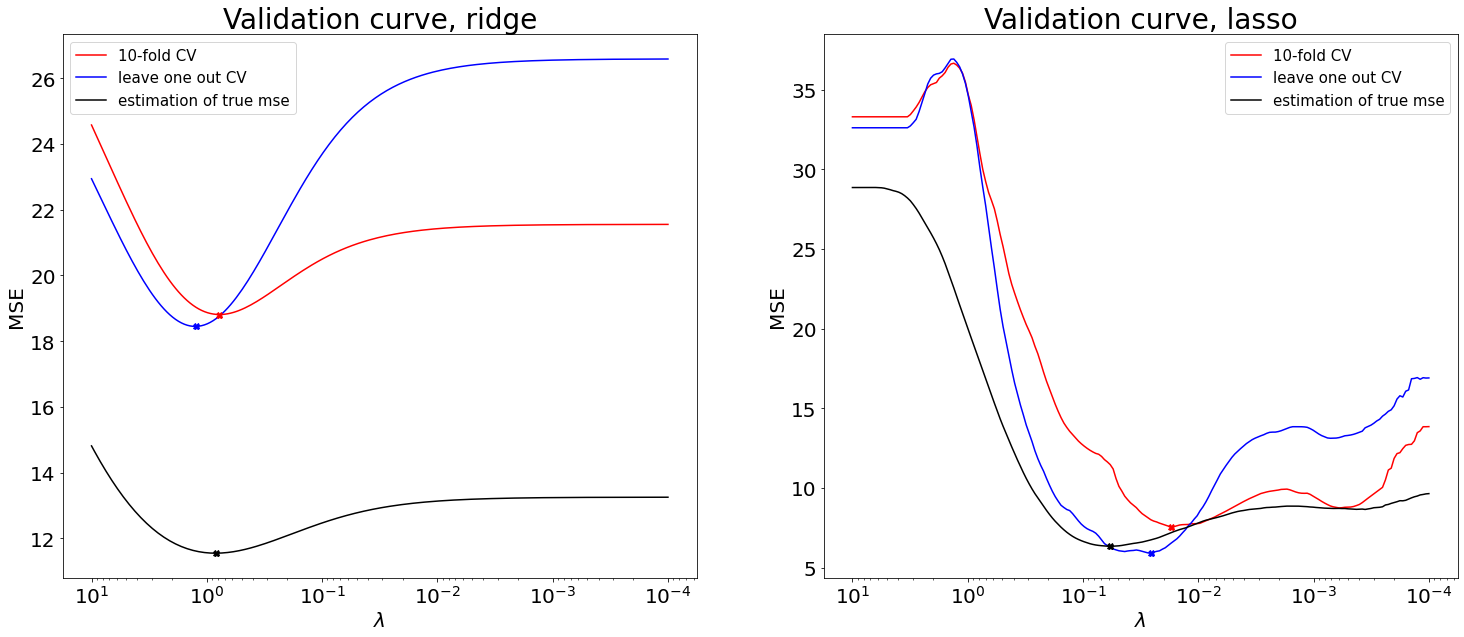
\includegraphics[scale=0.27]{Img/CV_simulation.png}%\hspace{-1.2cm}
        \centering
    \end{figure}
\end{frame}
%---------------------------------------------------------------------------%

